\title{Covariant Phase Space via MultiSymplectic Geometry}
\author{
        Antonio Michele Miti \\
                Department of Mathematics and Physics\\
        Università Cattolica del Sacro Cuore\\
        via Musei X, Brescia xxx, \underline{Italy}
}
\date{\today}

\documentclass[a4paper,12pt]{scrartcl}  %Per La Stampa
\usepackage[a4paper, margin=2cm]{geometry}

\usepackage{amsmath}
\usepackage[multisym, geomec,basic]{../Math-Symbols-List/commonmathsymb}
\usepackage{standalone}
\usepackage{graphicx}
\usepackage{wrapfig}

\input{../Latex-Theorem/TheoremTemplateToninus.tex}

	\renewcommand{\AffDualJet}{ J^{1 \TwistedAffine}E }
	\renewcommand{\LinDualJet}{ \overrightarrow{J^{1 \TwistedLinear}E} }


\begin{document}
\maketitle

\begin{abstract}
This is the paper's abstract \ldots
\end{abstract}

\section{Introduction}
Let's briefly recall in what consists the multisymplectic approach to mechanics of field systems in order to understand its relationship with the covariant phase space approach.

\begin{figure}
  \centering
  \includestandalone[mode=buildnew]{ms_landscape}
  \caption{multisymplectic landscape at glance}
\end{figure}

\begin{itemize}
 \item the starting point is the \emph{configuration bundle} 
 	\begin{displaymath}
 		E = \left( \pi_{M,E} : E\rightarrow M \right)
 	\end{displaymath}
 	the object encoding the kinematics.
 \item from that we have constructed the \emph{I jet bundle} applying the jet functor to $E$ 
 	\begin{displaymath}
 	J^1E = \left( \pi_{J^1 M,E} : J^1 E\rightarrow E \right)
 	\end{displaymath} 
 	that is an affine bundle over $E$.
 \item Then, we considered other two vector bundle derived from the first jet:
 	\begin{displaymath}
 	\AffDualJet  = \left( \pi_{ \AffDualJet ,E} : \AffDualJet  \rightarrow E \right)
 	\end{displaymath}
	twisted affine dual of $J^1E$ called \emph{"extended multiphase space"}.
	\begin{displaymath}
		\LinDualJet  = \left( \pi_{ \LinDualJet ,E} : \LinDualJet \rightarrow E \right)
	\end{displaymath}
	twisted linear dual of $J^1 E$ called \emph{"standard multiphase space"}. \footnote{It can be seen as the dual bundle of the vector bundle $\vec{J^1E}$ linear model of $J^1E$}
	The first one can be also seen as an affine line bundle over the second one.
	
\item It turns out that  $\LinDualJet $ carries a naturally defined multisymplectic form $\omega = -\textrm{d} \theta$ derived by a multicanonical m-form $\theta$. \\
	(This has been obtained pulling back the tautological m-form $\theta_\Lambda$ from $\bigwedge^m (E)$.) \\
	Thus, it can be considered the theoretical analogue of the cotangent bundle in ordinary geometric mechanics.
	
\item The dynamics can be implemented in two alternative way, fixing a further structure.\\
	In the Lagrangian picture is fixed a bundle map:
	\begin{displaymath}
		\Lagrangian : J^1 E \rightarrow \bigwedge^m (M)
	\end{displaymath}
	while in the Hamiltonian framework si fixed a section:
	\begin{displaymath}
		\Hamiltonian : \LinDualJet \rightarrow \AffDualJet
	\end{displaymath}

\item Both of them determine a \emph{Legendre map} computed as a fiber derivative.
	Mainly we are interested  in
	\begin{displaymath}
		\mathbb{F} \Lagrangian : J^1 E \rightarrow \AffDualJet		
	\end{displaymath}
	The two dynamics function can be considered equivalent under the condition of \emph{hyper-regularity}\cite[chapter, p.~215]{Gimmsy}.

\item Via $\mathbb{F} \Lagrangian$ we can pull-back the canonical forms on $J^1 E$ to give the \emph{Poincarè - Cartan forms}
	\begin{displaymath}
		\theta_\Lagrangian = \mathbb{F} \Lagrangian^\ast \theta \qquad \omega_\Lagrangian = - \textrm{d} \theta_\Lagrangian
	\end{displaymath}
	and via $\Hamiltonian$ we can pull-back the canonical forms on $\LinDualJet$ to give the \emph{De Donder - Weyl forms}
	\begin{displaymath}
		\theta_\Hamiltonian = \Hamiltonian^\ast \theta \qquad \omega_\Hamiltonian = - \textrm{d} \theta_\Lagrangian
	\end{displaymath}
	
\item At last, are introduced the \emph{Euler-Lagrange map}
	\begin{displaymath}
		D_\Lagrangian : J^2 E \rightarrow V^\TwistedLinear E
	\end{displaymath}
	 a bundle-morphism acting on holonomic section submanifolds $\varphi(M)$ as:
	\begin{displaymath}
		\left\langle D_\Lagrangian(\varphi, \partial \varphi , \partial^2 \varphi) \right\vert \left. V \right\rangle = (j^1 \varphi)^\ast \left( j^1V \lrcorner \omega_\Lagrangian \right)
	\end{displaymath}
	 a bundle-morphism when evaluated on a vertical field $V$ on $E$. \\
	And the \emph{DeDonder-Weyl map}
	\begin{displaymath}
		D_\Hamiltonian : J^1\left(\LinDualJet \right) \rightarrow V^\TwistedLinear \left(\LinDualJet \right)
	\end{displaymath}
	acting on holonomic section submanifolds $(\varphi, \pi)(M)$ as:
	\begin{displaymath}
		\left\langle D_\Hamiltonian(\varphi, \pi, \partial \varphi , \partial \pi) \right\vert \left. V \right\rangle = (\varphi, \pi)^\ast \left( V \lrcorner \omega_\Hamiltonian \right)
	\end{displaymath}	
	when evaluated on a vertical field $V$ on $\LinDualJet$.
	
\item	
	Imposing the vanishing of this map on an holonomic section gives a condition which corresponds to the well-know motion equations when rapresented in coordinate.

\end{itemize}


\section{Covariant phase space approach}
The gist of the transition from the \emph{multi-symplectic approach} to the \emph{Covariant Functional Approach} - based on the \emph{Covariant Phase Space} - is basically to perform a change of perspective.\\
We have to move our attention from the bundles to the cross-sections on the bundles.

The smooth bundle $(F:\rightarrow M)$ to be considered depends on the dynamical framework we are employing:

\begin{center}
\begin{tabular}{|c|c|c|}
	\hline
	 & Lagrangian picture & Hamiltonian picture \\
	\hline
	$F$		&	$E$		&	$\LinDualJet$	\\
	$\downarrow$ & $\downarrow$ & $\downarrow$ \\
	$M$ & $M$ & $M$ \\
	    & \emph{configuration bundle} & \emph{multiphase bundle} \\
	\hline
\end{tabular}
\end{center}

In this approach there are two central objects:

	\begin{definition}[Space of kinematics (off-shell) configurations]\label{Def:ConfSpace}
		Is the, generally non-linear, infinte-dimensional manifold :
		\begin{displaymath}
			\Conf \coloneqq \Gamma^\infty(F,M)
		\end{displaymath}
	\end{definition}
	
	\begin{definition}[Space of Dynamics (on-shell) configurations]\label{Def:SolSpace}
		Is the subset of $\Conf$:
		\begin{displaymath}
			\Sol \coloneqq \ker(D_\cdot) \subset \Conf
		\end{displaymath}
		containing all the smooth solutions of the motion equations corresponding to the  dynamical operator $D_\cdot$.
	\end{definition}

The key point of the latter definition is that the \emph{Euler-Lagrange} map and the \emph{DeDonder-Weyl} map, being bundle-morphism, can be regarded as mapping from $\Conf$ to the section of a suitable vector bundle.
They have to be composed with the jet functor $j^1$.

\begin{equation}
	D_\Lagrangian[\; ] = D_\Lagrangian \circ j^2 : \quad \Gamma^\infty(E) \ni \varphi \quad \mapsto \quad D_\Lagrangian[j^2 \varphi ] \in \Gamma^\infty \left( \phi^\ast \left(V^\TwistedLinear E \right)\right)
\end{equation}

\begin{equation}
	D_\Hamiltonian[\; ] = D_\Hamiltonian \circ j^1 : \quad \Gamma^\infty(F) \ni (\varphi,\pi) \quad \mapsto \quad D_\Hamiltonian[j^1 (\varphi,\pi) ] \in \Gamma^\infty \left( (\varphi,\pi)^\ast \left(V^\TwistedLinear F \right)\right)
\end{equation}

The target base is a vector space, more precisely a frechet space \cite[Cap.2]{Ban} and makes sense to ask whetever $D_\cdot [\phi]$ is equal to the 0-section.

\begin{notationfix}
Noticing the recurring scheme we will make use of the following notation:
	\begin{displaymath}
		W = V^\TwistedLinear F \; ; \; V = \Gamma^\infty(W,F) \quad \Rightarrow \quad D[\phi] \in V \quad \forall \phi \in \Conf
	\end{displaymath}
\end{notationfix}

The remarkable feature of the $\Sol$ space is that it carries a naturally defined pre-symplectic form $\Omega$. Natural beside the fact that its very structure, as a set, is expicitly determined by the fixed Lagrangian or Hamiltonian.\\
Therefore, is the candidate to  be the field-theoretic (Covariant) phase space.

Since $\Conf$ and $\Sol$ are in general not linear, we have to regard them as a manifold.
Hence, we have to specify conveniently the structure of their tangent space in order to make clair the preceeding claim.

The first thing to point out is the following chain of inequalities:
\begin{equation}
	\Gamma^\infty_c\left(\phi^*(VF)\right) \; \subseteq \; T_\phi\Sol \; \subset \; T_\phi\Conf \; \subseteq \; \Gamma^\infty\left( \phi^\ast (VF) \right)
\end{equation}

\begin{wrapfigure}{L}{0.50\textwidth}
\centering
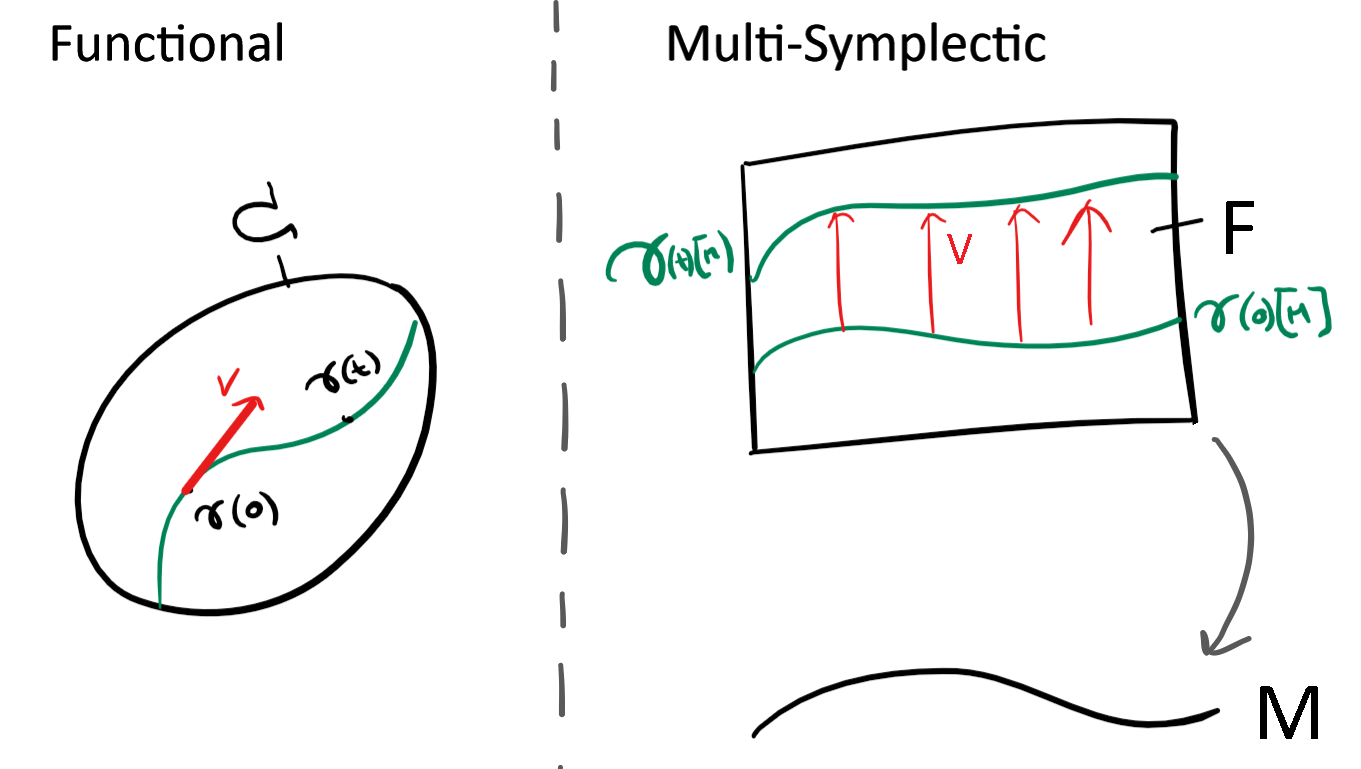
\includegraphics[width=0.49\textwidth]{Pictures/variations.png}
%\caption{\label{fig:variations}Covariant tangent fields as regular variations.}
\end{wrapfigure}

This condition stems from the fact that we want to interpret regular curves on $\Conf$ as smooth variations of field configurations. \\
Therefore, a parametrized regular curve as to be regarded as a family of diffeomerphisms, the flow generated by a vertical tangent field on $F$.\\
The pull-back are there to remark that $T_\phi \Conf$ consists of the infinitesimal smooth variations of $\phi$ thus are vertical field of $F$ \underline{along} the section $\phi$.

According to this interpretation, $T_\phi\Sol$ should consits of the generators of those variations that maps, at least infinitesimally, a solution $\phi\in\Sol$ in another solution.
A rigourosly, this can be expressed in the following definition:

	\begin{definition}[Tangent space to the Space of Solutions]\label{Def:TangentSol}
		\begin{displaymath}
			T_\phi \Sol \coloneqq \ker(J[\phi]_\cdot) \qquad \phi \in \Sol
		\end{displaymath}
	\end{definition}
In other words, it consists of the solutions of the Jacobi equations.

\section{Jacobi Operator}\label{Sec:JacobiOperator}
Intuitively, the Jacobi equation are the formal linearizazion of the motion equation around a solution $\phi$.\\
Precisely this can be encoded in the following operator:

	\begin{definition}[Jacobi operator pertaining to $D_\cdot$ around a solution $\phi \in \Sol$]\label{Def:JacobiOp}
		\begin{displaymath}
			J[\phi] \; : \; T_\phi \Conf \rightarrow	\phi^\ast(V^\TwistedLinear F) \quad s.t. \quad \left\langle D[\phi] \right.\left| \delta\phi \right\rangle
			= \sigma \left( \left.\dfrac{\textrm{d}}{\textrm{d} \lambda} D_\cdot [\phi_\lambda]\right\rvert_{\lambda=0} \right)
		\end{displaymath}
	\end{definition}

\begin{wrapfigure}{L}{0.41\textwidth}
\centering
\includegraphics[width=0.40\textwidth]{Pictures/jacobi.png}
\caption{\footnotesize \label{fig:jacobi}$J[\phi]$ and $D$ target on the same space.}
\end{wrapfigure}
where:
\begin{itemize}
	\item $\phi_\lambda$ is an arbitrary variation of $\phi_0 = \phi$ generated by $\delta\phi$.
	\item exactly as noted for the tangent vector of $\Conf$, we have for any $x\in M$:
		\begin{displaymath}
			\left.\dfrac{\textrm{d}}{\textrm{d} \lambda} D_\cdot [\phi_\lambda]\right\rvert_{\lambda=0}(x) \in V_M W
			\quad \Rightarrow \quad
			\left.\dfrac{\textrm{d}}{\textrm{d} \lambda} D_\cdot [\phi_\lambda]\right\rvert_{\lambda=0} \in D[\phi]^\ast \left( V_M \left( V^\TwistedLinear \right)\right)
		\end{displaymath}
		because $D_\cdot[\phi_\lambda]$ can be regarded as a section of $V^\TwistedLinear F$ over $M$, 
		thus the latter definition does not depend from the particular choice of variation $\phi_\lambda$ 
		but only from its infinitesimal generator $\delta\phi$.
	\item $\sigma$ is the canonical bundle-morphism
		\begin{displaymath}
			\sigma:  0^\ast \left( V_M W \right)  \; \rightarrow \;  0^\ast \left(V_E W \right) \simeq W
		\end{displaymath}
		 where $V_M W$ and $V_F W$ are the vertical sub-bundle of $T W$ w.r.t. $M$ and $F$ respectively 
		 and $0$ is the zero-section of $W$ over $F$.
\end{itemize}

The operator is well defined since
\begin{displaymath}
	\phi \in \Sol \quad \Rightarrow \quad D[\phi] \subset 0(E)
\end{displaymath}

\section{Construction of $\sigma$}
Consider the two stacked bundle, $ W \rightarrow E$ vector bundle, $E \rightarrow M$ smooth bundle.

where $m$ is the standard bundle morphism of pull-back bundle:
\begin{displaymath}
	m : \left( \pi^\ast \left( T E \right) \right)_w = \{w\} \times \{T_{\pi(w)} \} \mapsto T_{\pi(w)} E
\end{displaymath}

\begin{figure}
  \centering
  \includestandalone[mode=buildnew]{ms_sigmaconstruction}
\end{figure}

We have the following short exact sequence of bundle morphism over $W$
\begin{figure}
  \centering
  \caption{short exact sequence}
\end{figure}
because

\begin{displaymath}
	\ker(i) = 0 (E) = i' \left( 0 \right)
\end{displaymath}
\begin{displaymath}
	\ker\left( T \pi_{E,W} \right) = V_E W = i\left( V_E W \right)
\end{displaymath}
\begin{displaymath}
	\ker\left(T \pi_{M,E}\right) = V_M E = T \pi_{E,W} \left( V_M W \right)
\end{displaymath}

We can exhibit a right splitting, that is:
\begin{displaymath}
	u : C \rightarrow B \quad \textrm{s.t.} \quad u \circ T \pi_{E,W} = \textrm{id}_B
\end{displaymath}
so, by splitting lemma, we have a left splitting $\sigma : B \rightarrow A$.

The claimed right splitting is the following:
\begin{align*}
		u = T0 \circ m \; : & \; \pi^\ast_{E,W} \left(TE \right) \rightarrow TE \rightarrow TW \\
						& \{w\} \times \{V_{\pi(w)} \} \mapsto V_{\pi(w)} \mapsto \left( T_{\pi(w)}0\right) (V_{\pi(w)})
\end{align*}



\paragraph{Outline}
The remainder of this article is organized as follows.
Section~\ref{previous work} gives account of previous work.
Our new and exciting results are described in Section~\ref{results}.
Finally, Section~\ref{conclusions} gives the conclusions.



\begin{figure}
  \centering
  \includegraphics{Pictures/jacobi.png}
  \caption{.}
\end{figure}

\begin{figure}
  \centering
  \includegraphics{Pictures/jacobi.png}
  \caption{.}
\end{figure}

\begin{figure}
  \centering
  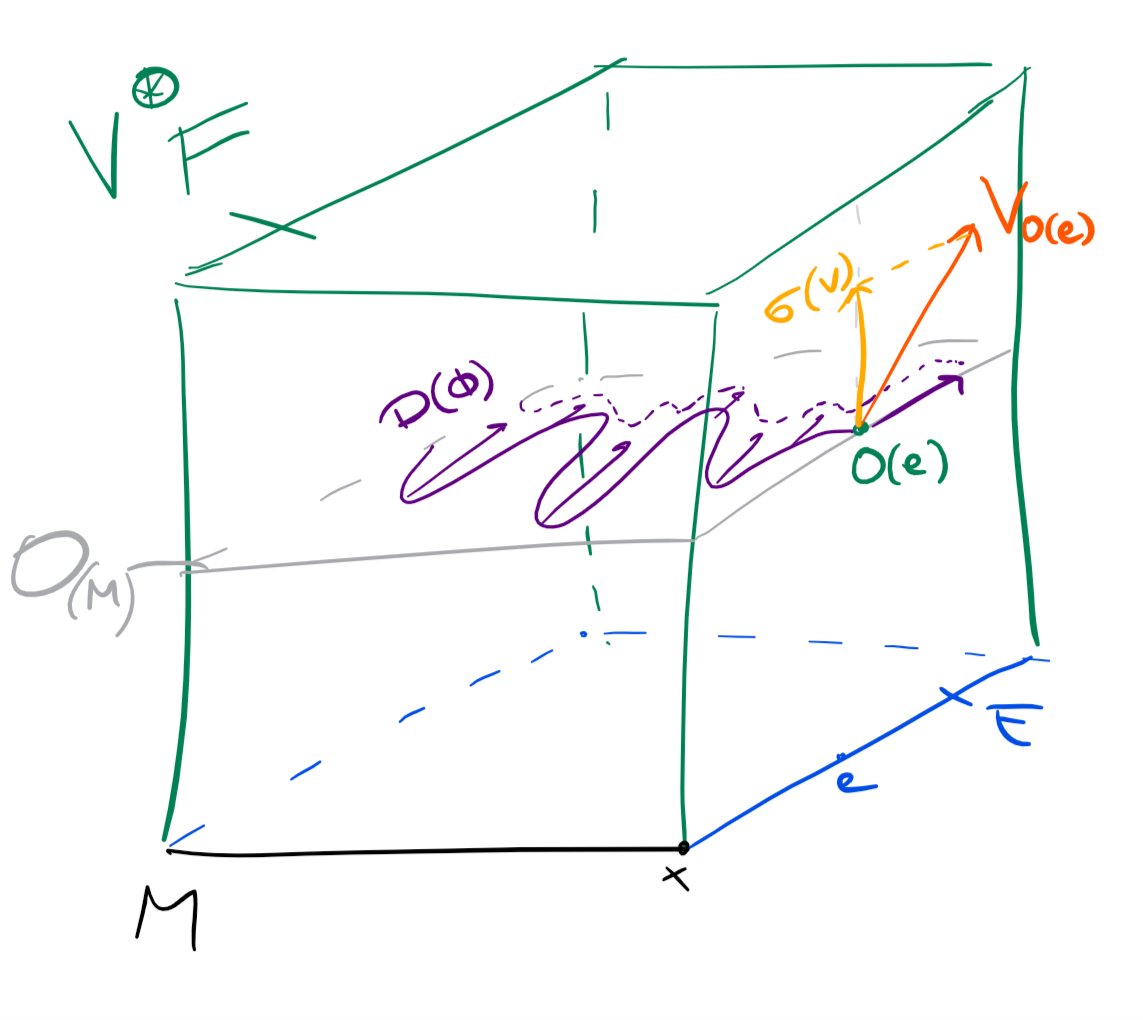
\includegraphics{Pictures/fieldJacobi.png}
  \caption{.}
\end{figure}

\begin{figure}
  \centering
  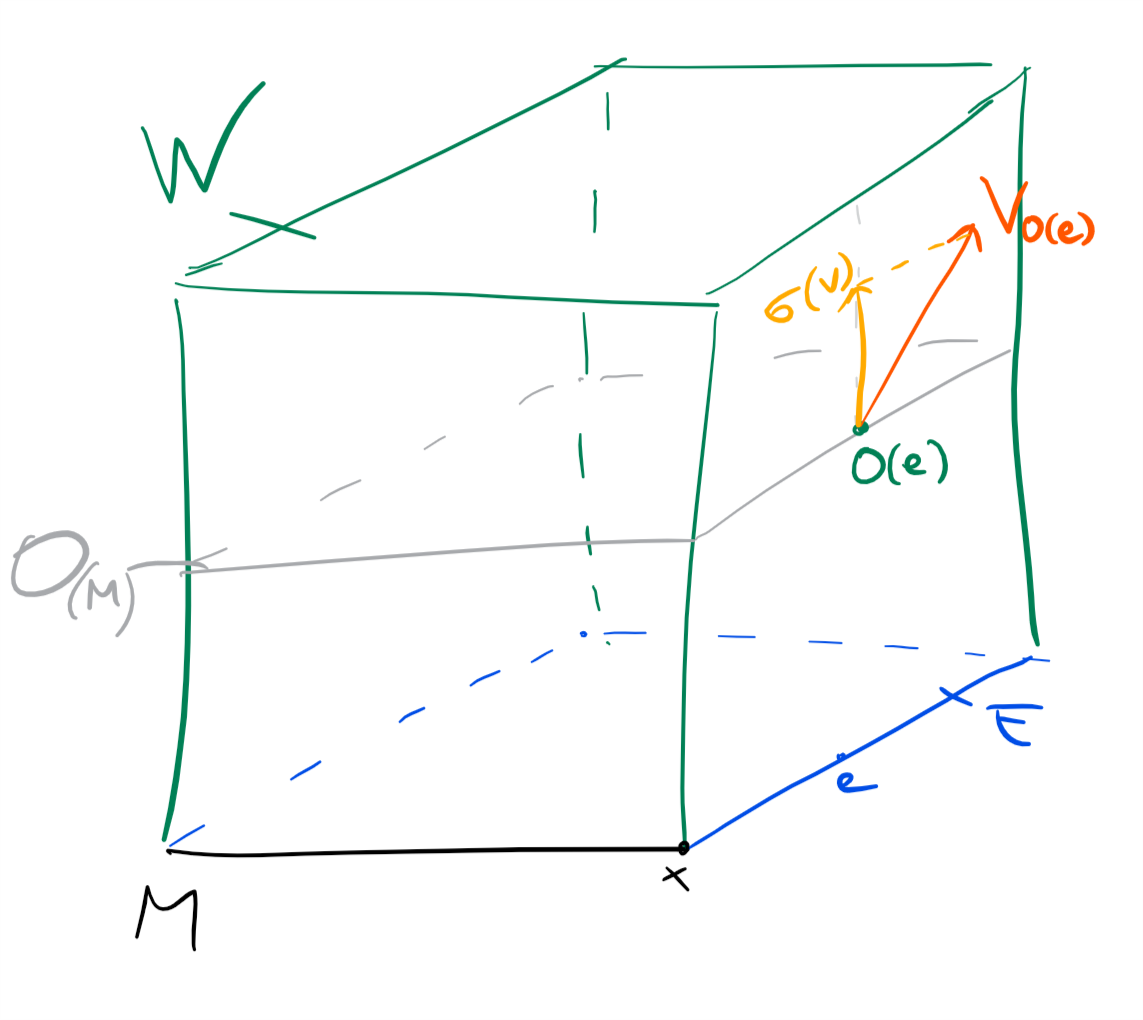
\includegraphics{Pictures/sigma.png}
  \caption{.}
\end{figure}



\bibliographystyle{abbrv}
\bibliography{main}
\begin{thebibliography}{9}

\bibitem{Gimmsy}
  Leslie Lamport,
  \emph{\LaTeX: a document preparation system},
  Addison Wesley, Massachusetts,
  2nd edition,
  1994.

\end{thebibliography}

\end{document}
